\chapter{From a Particle in a Box to Bloch States}
\label{ch:particle-box-to-bloch}

A quantum particle confined to a finite region has a discrete spectrum.  A
particle in a periodic crystal also has discrete states when the crystal is
finite, but lattice translation organizes those states by a Bloch wave vector.
This chapter develops that connection from boundary conditions, translation
symmetry, and the spectral representation of the one-electron Hamiltonian
\cite{kittel2005,yu2010,rudan2015}.

\section{The one-dimensional infinite box}

Consider one electron on the interval $0<x<L$ with infinitely high walls.  The
Hamiltonian inside the box is
\begin{equation}
  \hat H
  =-\frac{\hbar^2}{2m}\frac{\dd^2}{\dd x^2},
  \label{eq:box-hamiltonian}
\end{equation}
and its domain imposes
\begin{equation}
  \psi(0)=\psi(L)=0.
  \label{eq:box-dirichlet-boundary-conditions}
\end{equation}
The stationary Schrödinger equation is
\begin{equation}
  -\frac{\hbar^2}{2m}\frac{\dd^2\psi}{\dd x^2}
  =E\psi.
  \label{eq:box-stationary-schrodinger}
\end{equation}
For $E>0$, define
\begin{equation}
  k=\frac{\sqrt{2mE}}{\hbar}.
  \label{eq:box-wave-number-energy}
\end{equation}
The general interior solution is
\begin{equation}
  \psi(x)=A\sin(kx)+B\cos(kx).
  \label{eq:box-general-solution}
\end{equation}
The boundary condition at $x=0$ gives $B=0$.  The condition at $x=L$ gives
\begin{equation}
  \sin(kL)=0,
  \label{eq:box-quantization-condition}
\end{equation}
so
\begin{equation}
  k_n=\frac{n\pi}{L},
  \qquad n=1,2,3,\ldots.
  \label{eq:box-allowed-wave-numbers}
\end{equation}
Normalization produces
\begin{equation}
  \boxed{
  \phi_n(x)=\sqrt{\frac{2}{L}}
  \sin\left(\frac{n\pi x}{L}\right),
  }
  \label{eq:box-normalized-eigenfunctions}
\end{equation}
and the energies are
\begin{equation}
  \boxed{
  E_n=\frac{\hbar^2\pi^2n^2}{2mL^2}.
  }
  \label{eq:box-energy-spectrum}
\end{equation}

The discrete spectrum follows from the boundary conditions.  Each allowed
standing wave must contain an integer number of half wavelengths inside the
box:
\begin{equation}
  L=n\frac{\lambda_n}{2}.
  \label{eq:box-half-wavelength-count}
\end{equation}
The finite length selects a discrete set of wavelengths and therefore a
discrete set of energies.

\begin{figure}[H]
  \centering
  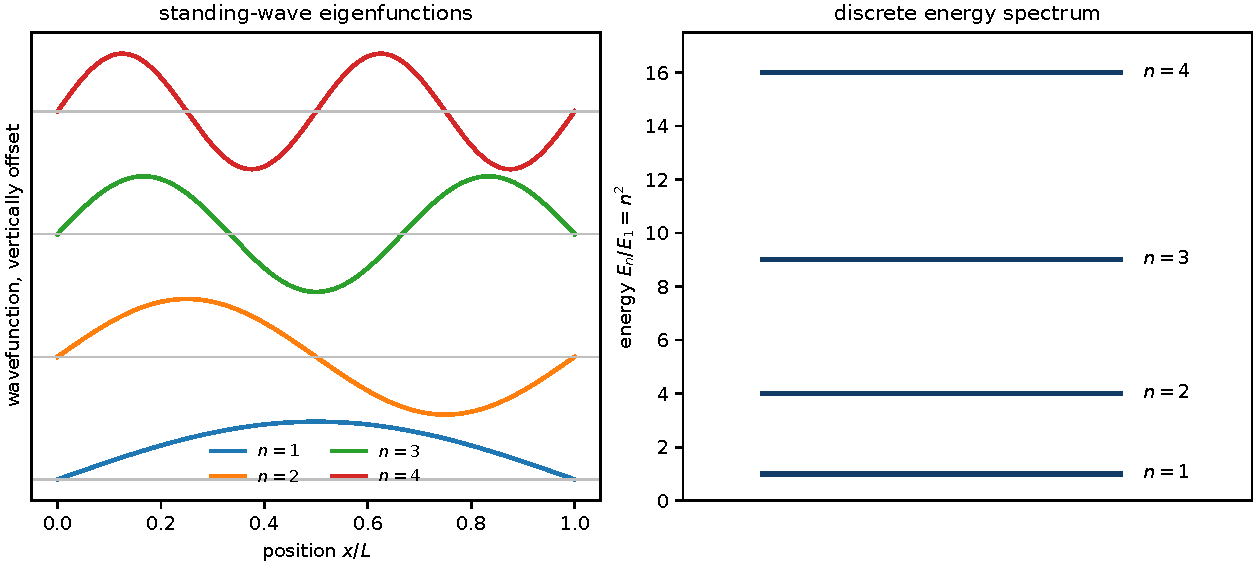
\includegraphics[width=0.88\textwidth]{figures/foundation-piab-spectrum.pdf}
  \caption{The first four particle-in-a-box eigenfunctions and their energies.
  The number of interior nodes increases with $n$, while the spectrum grows as
  $n^2$.\figurenotebookmark}
  \label{fig:foundation-piab-spectrum}
\end{figure}
\figurenotebooktext{figures/01_particle-box-to-bloch/fig_01_01.ipynb}

\section{Spectral representation of the box Hamiltonian}

The eigenfunctions form an orthonormal basis:
\begin{equation}
  \braket{m|n}=\delta_{mn},
  \label{eq:box-orthonormality}
\end{equation}
and resolve the identity on the box Hilbert space:
\begin{equation}
  \hat I=\sum_{n=1}^{\infty}\ket{n}\bra{n}.
  \label{eq:box-completeness}
\end{equation}
The Hamiltonian has the spectral representation
\begin{equation}
  \boxed{
  \hat H=\sum_{n=1}^{\infty}E_n\ket{n}\bra{n}.
  }
  \label{eq:box-hamiltonian-spectral-representation}
\end{equation}
An arbitrary state expands as
\begin{equation}
  \ket{\psi}=\sum_{n=1}^{\infty}c_n\ket{n},
  \qquad
  c_n=\braket{n|\psi}.
  \label{eq:box-state-expansion}
\end{equation}
The probability of measuring $E_n$ is
\begin{equation}
  \mathbb P(E_n)=|c_n|^2.
  \label{eq:box-energy-measurement-probability}
\end{equation}
This finite-region example establishes the main spectral objects: eigenvalues,
eigenstates, projectors, and multiplicities.

\section{Periodic boundary conditions and plane waves}

Replace the hard walls by the periodic condition
\begin{equation}
  \psi(x+L)=\psi(x).
  \label{eq:ring-periodic-boundary-condition}
\end{equation}
The free-particle eigenfunctions are plane waves
\begin{equation}
  \phi_k(x)=\frac{1}{\sqrt L}e^{ikx}.
  \label{eq:ring-plane-wave}
\end{equation}
Periodicity requires
\begin{equation}
  e^{ikL}=1,
  \label{eq:ring-phase-quantization}
\end{equation}
which gives
\begin{equation}
  \boxed{
  k_m=\frac{2\pi m}{L},
  \qquad m\in\mathbb Z.
  }
  \label{eq:ring-wave-vector-quantization}
\end{equation}
The energies are
\begin{equation}
  E_m=\frac{\hbar^2k_m^2}{2m}.
  \label{eq:ring-free-particle-energies}
\end{equation}
The spacing of neighboring wave vectors is
\begin{equation}
  \Delta k=\frac{2\pi}{L}.
  \label{eq:ring-k-spacing}
\end{equation}
As $L$ grows, the discrete wave vectors become dense while the state density
$L/(2\pi)$ per unit $k$ remains finite.

The hard-wall box uses standing waves because reflection fixes nodes at two
boundaries.  The periodic box uses traveling waves because translation through
$L$ returns the same state.  Both spectra are discrete for finite $L$; their
boundary conditions organize the eigenstates differently.

\begin{figure}[H]
  \centering
  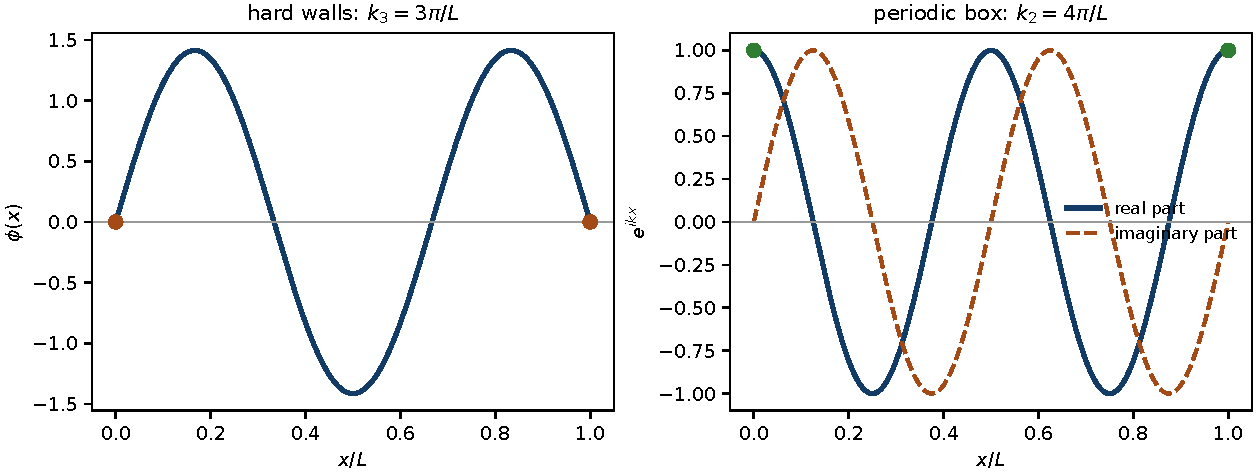
\includegraphics[width=0.84\textwidth]{figures/foundation-boundary-conditions.pdf}
  \caption{Hard-wall and periodic boundary conditions select different
  eigenfunctions.  The hard-wall box supports standing waves with
  $k_n=n\pi/L$; the periodic box supports plane waves with
  $k_m=2\pi m/L$.\figurenotebookmark}
  \label{fig:foundation-boundary-conditions}
\end{figure}
\figurenotebooktext{figures/01_particle-box-to-bloch/fig_01_02.ipynb}

\section{Translation as a symmetry}

The translation operator through a displacement $a$ acts as
\begin{equation}
  (\hat T_a\psi)(x)=\psi(x+a).
  \label{eq:translation-operator-action}
\end{equation}
Successive translations satisfy
\begin{equation}
  \hat T_a\hat T_b=\hat T_{a+b}.
  \label{eq:translation-group-composition}
\end{equation}
For a periodic potential,
\begin{equation}
  V(x+a)=V(x),
  \label{eq:periodic-potential}
\end{equation}
the Hamiltonian
\begin{equation}
  \hat H
  =-\frac{\hbar^2}{2m}\frac{\dd^2}{\dd x^2}+V(x)
  \label{eq:periodic-one-electron-hamiltonian}
\end{equation}
commutes with lattice translation:
\begin{equation}
  [\hat H,\hat T_a]=0.
  \label{eq:hamiltonian-translation-commutator}
\end{equation}
Energy eigenstates can therefore be chosen as translation eigenstates:
\begin{equation}
  \hat T_a\psi_k=\lambda_k\psi_k.
  \label{eq:translation-eigenvalue-equation}
\end{equation}
Translation preserves normalization, so $|\lambda_k|=1$.  Write
\begin{equation}
  \lambda_k=e^{ika}.
  \label{eq:translation-eigenvalue-phase}
\end{equation}
The eigenvalue equation becomes
\begin{equation}
  \boxed{
  \psi_k(x+a)=e^{ika}\psi_k(x).
  }
  \label{eq:bloch-boundary-condition}
\end{equation}

\section{Bloch's theorem}

Define
\begin{equation}
  u_k(x)=e^{-ikx}\psi_k(x).
  \label{eq:bloch-periodic-part-definition}
\end{equation}
Using \cref{eq:bloch-boundary-condition},
\begin{equation}
\begin{aligned}
  u_k(x+a)
  &=e^{-ik(x+a)}\psi_k(x+a)\\
  &=e^{-ikx}e^{-ika}e^{ika}\psi_k(x)\\
  &=u_k(x).
\end{aligned}
  \label{eq:bloch-periodic-part-proof}
\end{equation}
Thus $u_k$ has the lattice period and
\begin{equation}
  \boxed{
  \psi_{nk}(x)=e^{ikx}u_{nk}(x),
  \qquad u_{nk}(x+a)=u_{nk}(x).
  }
  \label{eq:bloch-theorem-one-dimensional}
\end{equation}
The band index $n$ distinguishes different eigenstates at the same $k$.

Substitution into the Schrödinger equation gives the cell-periodic eigenproblem
\begin{equation}
  \boxed{
  \hat H(k)u_{nk}=E_n(k)u_{nk},
  }
  \label{eq:bloch-cell-periodic-eigenproblem}
\end{equation}
with
\begin{equation}
  \hat H(k)
  =e^{-ikx}\hat H e^{ikx}
  =\frac{(\hat p+\hbar k)^2}{2m}+V(x).
  \label{eq:bloch-hamiltonian-k}
\end{equation}
For each $k$, diagonalization of $\hat H(k)$ gives the band energies
$E_n(k)$.

\begin{figure}[H]
  \centering
  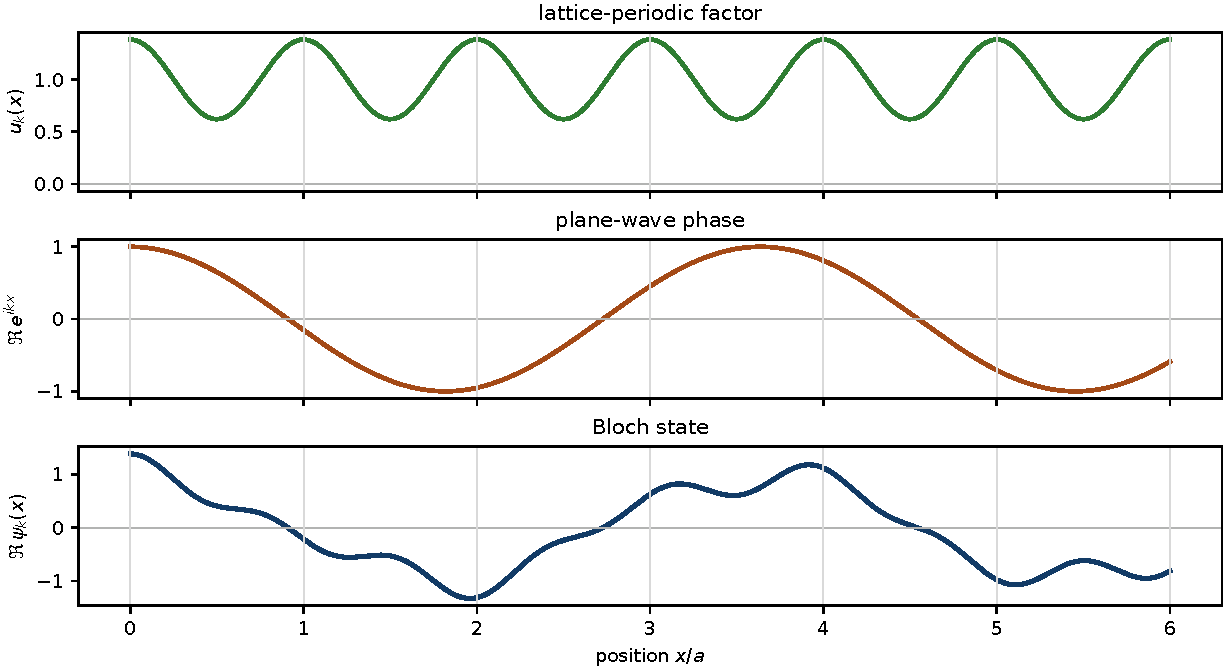
\includegraphics[width=0.88\textwidth]{figures/foundation-bloch-wave.pdf}
  \caption{A Bloch state is the product of a plane-wave phase and a
  lattice-periodic function.  Translation through one cell changes the full
  state by the phase $e^{ika}$ while reproducing the periodic factor.\figurenotebookmark}
  \label{fig:foundation-bloch-wave}
\end{figure}
\figurenotebooktext{figures/01_particle-box-to-bloch/fig_01_03.ipynb}

\section{A finite crystal selects discrete Bloch wave vectors}

Let the crystal contain $N$ cells, so $L=Na$, and impose periodicity across the
whole crystal:
\begin{equation}
  \psi_k(x+Na)=\psi_k(x).
  \label{eq:finite-crystal-periodicity}
\end{equation}
Repeated application of Bloch's condition gives
\begin{equation}
  \psi_k(x+Na)=e^{ikNa}\psi_k(x).
  \label{eq:repeated-bloch-translation}
\end{equation}
Therefore
\begin{equation}
  e^{ikNa}=1,
  \label{eq:finite-crystal-k-condition}
\end{equation}
and
\begin{equation}
  k_m=\frac{2\pi m}{Na}.
  \label{eq:finite-crystal-bloch-k}
\end{equation}
There are $N$ distinct $k$ values in one Brillouin zone for each band.  This
matches the $N$ primitive cells in the finite crystal.

A reciprocal-lattice vector in one dimension is
\begin{equation}
  G=\frac{2\pi\ell}{a},
  \qquad \ell\in\mathbb Z.
  \label{eq:one-dimensional-reciprocal-lattice}
\end{equation}
The translation phase is unchanged by $k\rightarrow k+G$:
\begin{equation}
  e^{i(k+G)a}=e^{ika}e^{i2\pi\ell}=e^{ika}.
  \label{eq:bloch-k-reciprocal-equivalence}
\end{equation}
Distinct crystal momenta can therefore be represented in the first Brillouin
zone,
\begin{equation}
  -\frac{\pi}{a}\le k<\frac{\pi}{a}.
  \label{eq:first-brillouin-zone-one-dimensional}
\end{equation}

\section{Three-dimensional form}

For lattice vectors $\bm R$, Bloch's theorem becomes
\begin{equation}
  \psi_{n\bm k}(\bm r+\bm R)
  =e^{i\bm k\cdot\bm R}\psi_{n\bm k}(\bm r),
  \label{eq:bloch-translation-three-dimensional}
\end{equation}
or
\begin{equation}
  \psi_{n\bm k}(\bm r)
  =e^{i\bm k\cdot\bm r}u_{n\bm k}(\bm r),
  \qquad
  u_{n\bm k}(\bm r+\bm R)=u_{n\bm k}(\bm r).
  \label{eq:bloch-theorem-three-dimensional}
\end{equation}
Reciprocal vectors $\bm G$ satisfy
\begin{equation}
  e^{i\bm G\cdot\bm R}=1,
  \label{eq:reciprocal-lattice-definition}
\end{equation}
so $\bm k$ and $\bm k+\bm G$ represent the same lattice-translation character.
The first Brillouin zone contains one distinct $\bm k$ value per primitive cell
for each band in a finite periodic crystal.

\section{Chapter summary}

Hard-wall confinement converts the free-particle continuum into discrete
standing-wave energies.  Periodic boundary conditions produce discrete plane
waves and a uniform reciprocal-space spacing.  A lattice-periodic Hamiltonian
commutes with translation, so its one-electron eigenstates carry translation
phases $e^{i\bm k\cdot\bm R}$.  Bloch's theorem separates each state into a
plane-wave factor and a lattice-periodic factor.  A finite crystal supplies one
allowed $\bm k$ value per primitive cell in each band.  The next chapter shows
how coupling localized orbitals produces those Bloch bands and connects finite
HOMO--LUMO spectra to bulk valence and conduction bands.
